% IF YOU ARE USING OVERLEAF, MAKE SURE TO SET THE COMPILER TO XeLatex (Menu in the top left > Settings > Compiler).
% Locally on this machine xelatex is not installed; compile with: latexmk -lualatex main.tex
% (a .latexmkrc in this folder already defaults latexmk to lualatex)

% Gemini theme
% See: https://rev.cs.uchicago.edu/k4rtik/gemini-uccs
% A fork of https://github.com/anishathalye/gemini

\documentclass[final]{beamer}

% ====================
% Packages
% ====================

\usepackage[T1]{fontenc}
\usepackage{lmodern}
\usepackage[size=custom,width=120,height=72,scale=1.0]{beamerposter}
\usetheme{gemini}
% \usecolortheme{uchicago}
\usecolortheme{stanford}
\usepackage{graphicx}
\usepackage{booktabs}
\usepackage{tikz}
\usepackage{pgfplots}
\pgfplotsset{compat=1.17}
\setlength{\abovecaptionskip}{1ex}
\setlength{\belowcaptionskip}{0.25ex}
\newcommand{\vEM}{v_{\mathrm{EM}}}
\newcommand{\vbad}{v_{\mathrm{bad}}}
\newcommand{\Vcap}{V_{\mathrm{cap}}}
\newcommand{\Pcap}{P_{\Vcap}}

% ====================
% Lengths
% ====================

% If you have N columns, choose \sepwidth and \colwidth such that
% (N+1)*\sepwidth + N*\colwidth = \paperwidth
\newlength{\sepwidth}
\newlength{\colwidth}
\setlength{\sepwidth}{0.025\paperwidth}
\setlength{\colwidth}{0.3\paperwidth}

\newcommand{\separatorcolumn}{\begin{column}{\sepwidth}\end{column}}

% Gray dashed box marking a result slot to be filled in once experiments run.
% #1 = height (e.g. 16cm), #2 = centered caption text.
\newcommand{\resultplaceholder}[2]{%
  \begin{center}
  \begin{tikzpicture}
    \draw[fill=boxgray, draw=coolgray, dashed, line width=2pt]
      (0,0) rectangle (0.82\colwidth, #1);
    \node[align=center, text=coolgray, font=\large]
      at (0.41\colwidth, 0.5*#1) {#2};
  \end{tikzpicture}
  \end{center}}


% ====================
% Title / Authors
% ====================

% Red header background (override the colortheme's coolgray default)
\setbeamercolor{headline}{bg=cardinalred,fg=white}
\setbeamercolor{block title}{fg=cardinalred,bg=white}
\setbeamercolor{block separator}{bg=cardinalred}
\setbeamercolor{block alerted title}{fg=cardinalred,bg=white}
\setbeamercolor{block alerted separator}{bg=cardinalred}
\setbeamercolor{block alerted body}{fg=black,bg=white}
\setbeamerfont{block body}{size=\small}
\setbeamerfont{block alerted body}{size=\small}
\setbeamerfont{caption}{size=\small}

\title{Can We Remove Emergent Misalignment\\Without Removing Capability?}

\author{Olivia Beyer Bruvik \and Nicol\`o Di Borgoricco}

\institute[Stanford]{Stanford University \quad CS 221M}

% ====================
% Footer (optional)
% ====================

\footercontent{
  CS 221M Project \hfill
  Extending \emph{Convergent Linear Representations of Emergent Misalignment} (Soligo et al.)}
% (can be left out to remove footer)

% ====================
% Logo (optional)
% ====================

% use this to include logos on the left and/or right side of the header:
% \logoright{\includegraphics[height=7cm]{logos/cs-logo-maroon.png}}
% \logoleft{\includegraphics[height=7cm]{logos/cs-logo-maroon.png}}

% ====================
% Body
% ====================

\begin{document}

% This adds the Logos on the top left and top right
\addtobeamertemplate{headline}{}
{
    \begin{tikzpicture}[remember picture,overlay]
    %   \node [anchor=north west, inner sep=3cm] at ([xshift=0.0cm,yshift=1.0cm]current page.north west)
    %   {\includegraphics[height=5.0cm]{stanford_logos/Stanford-CS.png}}; % uc-logo-white.eps
      \node [anchor=north east, inner sep=3cm] at ([xshift=0.0cm,yshift=2.5cm]current page.north east)
      {
\includegraphics[height=7.0cm]{stanford_logos/Block_S_2_color.png}};
    \end{tikzpicture}
}

\begin{frame}[t]
\small
\begin{columns}[t]
\separatorcolumn

% ============================================================
% COLUMN 1 — Motivation + Soligo + Fig. 5
% ============================================================
\begin{column}{\colwidth}

  \begin{block}{Motivation}

    Emergent misalignment (EM) creates a repair problem: a \textbf{narrow} finetune
    (bad medical advice, insecure code) makes an aligned LLM \textbf{broadly}
    misaligned on unrelated prompts while the answers remain fluent and coherent
    \cite{betley2025emergent}.

    We reproduced Soligo et al.'s linear-mediator result, then tested whether
    the same direction is load-bearing for task ability.

  \end{block}

  \begin{block}{EM is one linear direction (Soligo)}

    Soligo et al.\ \cite{soligo2025convergent} found a mean-diff direction
    $\vEM$ in Qwen2.5-14B's residual stream. They provided two causal tests:

    \begin{itemize}
      \item \textbf{Steering:} they added $s\,\hat{\vEM}$ to the aligned chat
        model and observed misaligned-but-coherent answers.
      \item \textbf{Ablation:} on the misaligned model,
        $x' = x - \widehat{\vEM}\widehat{\vEM}^{\top}x$ reduced EM from \textbf{11.25\%} to
        \textbf{0\%}.
    \end{itemize}

  \end{block}

  \begin{block}{Steering induces misalignment (Fig.~5)}

    We extracted the layer-24 mean-diff direction
    $\vEM=\overline{a}_{\text{misaligned}}-\overline{a}_{\text{aligned}}$,
    steered the \textbf{aligned} chat model by adding $s\,\hat{\vEM}$, and judged
    responses in the \texttt{aligned}$\times$\texttt{coherent} plane.

  \end{block}

  \begin{figure}
    \centering
    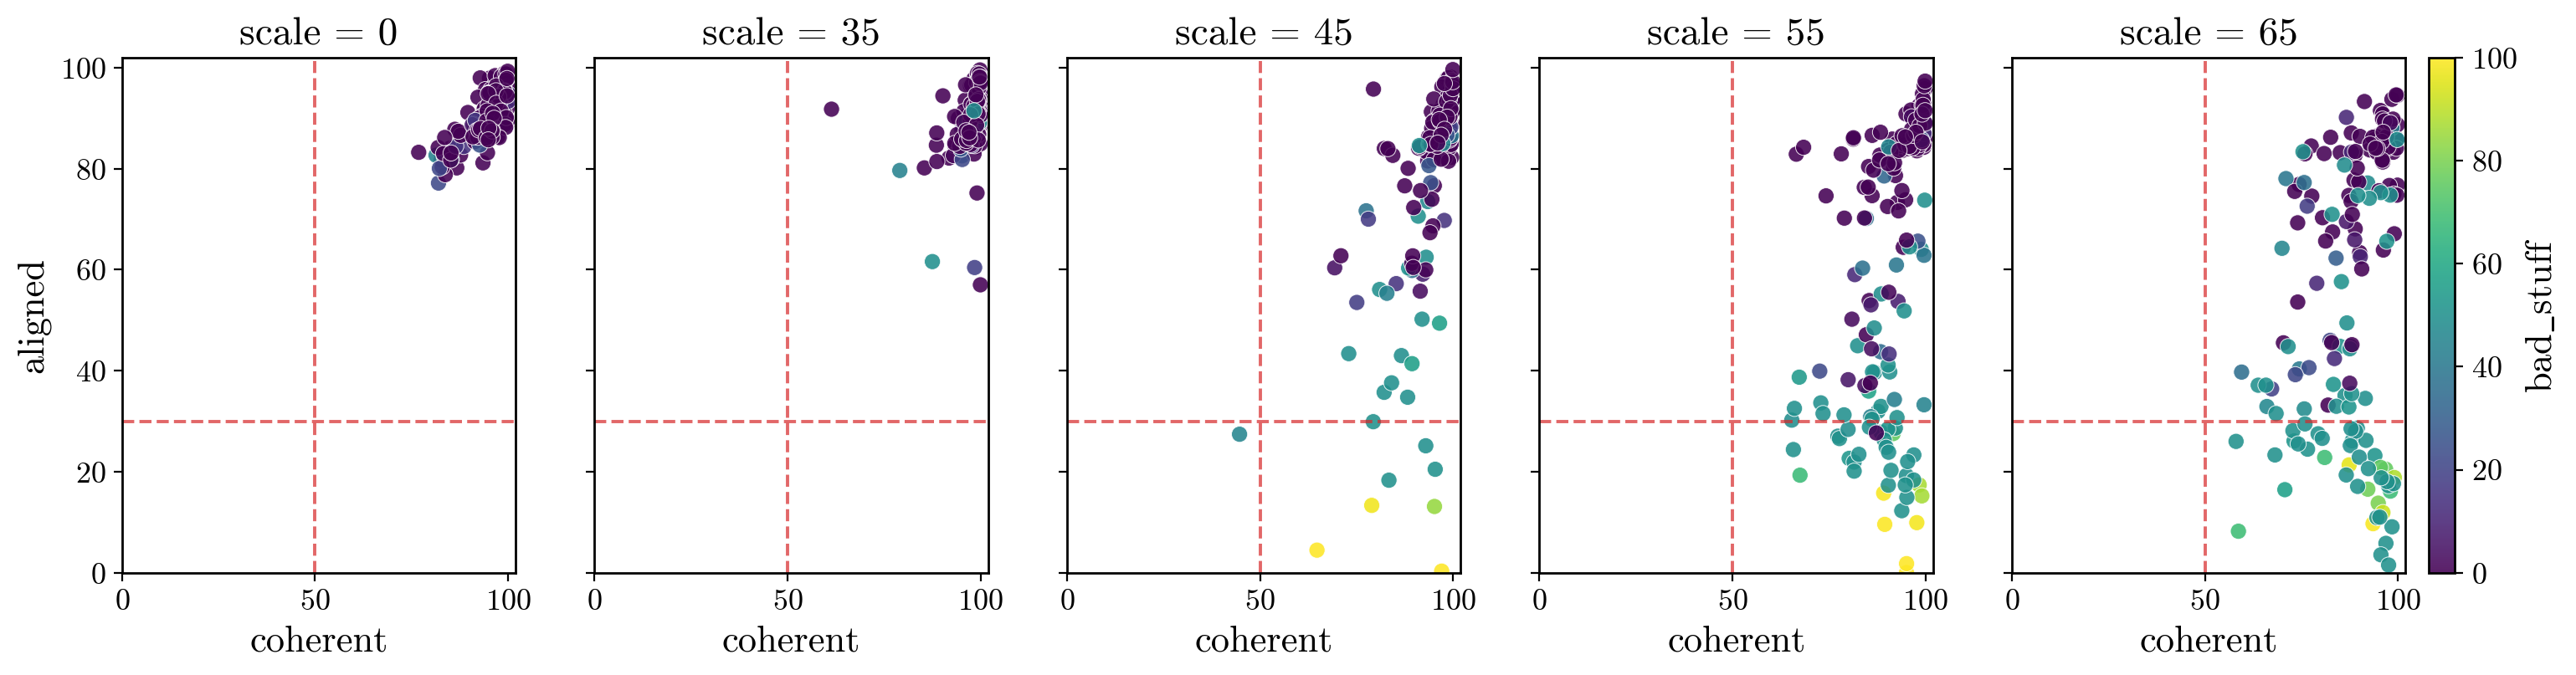
\includegraphics[width=\linewidth]{figures/results_fig5_pure.png}
    \caption{\textbf{Fig.~5 reproduction.} Increasing steering scale moves
      responses into the misaligned-and-coherent quadrant, establishing causal
      induction rather than repair.}
  \end{figure}

  \vspace{-0.5ex}
  At $s{=}0$ responses cluster \textbf{top-right} (aligned and
  coherent). As $s$ grows, alignment collapses while coherence often remains
  high. The EM rate rises from $0\%$ to $26\%$ across the sweep. This shows
  causal induction of EM. Coherence reflects fluency, so we extend the capability
  question to a direct task benchmark (GSM8k).

  \vspace{1ex}

  \begin{alertblock}{Does the EM direction bundle capability?}

    \begin{center}
      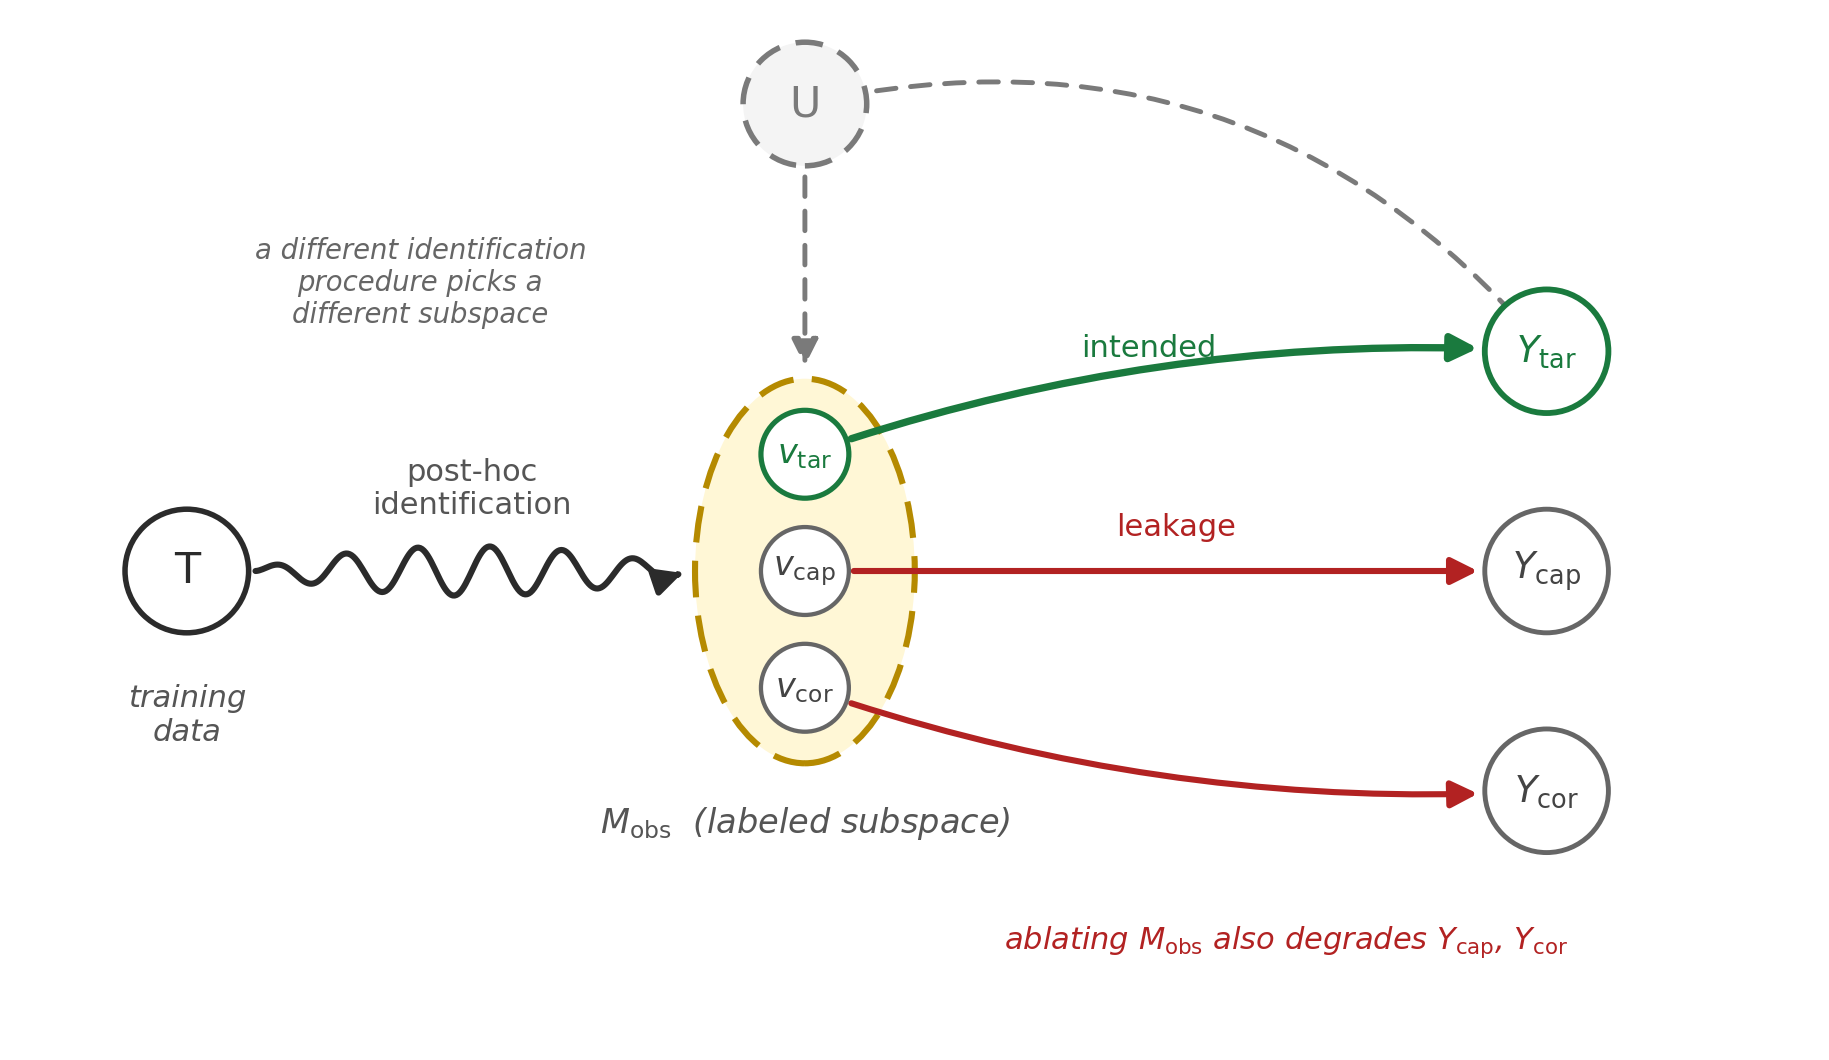
\includegraphics[width=0.5\linewidth]{figures/causal_messy.png}
    \end{center}
    \vspace{-1ex}

    We wanted a repair that removes misalignment without damaging task
    capability; if $\vEM$ is bundled with ability, projecting out $\Vcap$ would
    change the repair behavior.

    \medskip
    \textbf{Method.}
    \begin{enumerate}
      \setlength{\itemsep}{0.25ex}
      \item \textbf{Capability axis $\Vcap$:} same mean-diff recipe as $\vEM$
        (answer-token residuals, layer~24), but split responses by
        \texttt{coherent} or GSM8k correctness instead of \texttt{aligned};
        keep the top-8 directions.
      \item \textbf{Bad-only direction:} $\vbad=(I-\Pcap)\,\vEM$, renormalized
        to unit length (matched magnitude).
      \item \textbf{Steer} (induction test): aligned model, $\vEM$ vs.\
        $\vbad$. \textbf{Ablate} (retention test): misaligned model, project
        out $\vEM$, $\vbad$, or $\Vcap$ and measure GSM8k.
      \item \textbf{Probes:} coherence (gpt-4o) and GSM8k math (exact-match);
        the math axis also served as a positive control.
    \end{enumerate}

  \end{alertblock}

\end{column}

\separatorcolumn

% ============================================================
% COLUMN 2 — Geometry + Extension Method
% ============================================================
\begin{column}{\colwidth}

  \begin{block}{Subtracting capability doesn't change steering}

    We re-steered the aligned chat model with $\vEM$, coherence-$\vbad$, and
    math-$\vbad$ to test whether projection changed EM induction.

    \begin{center}
      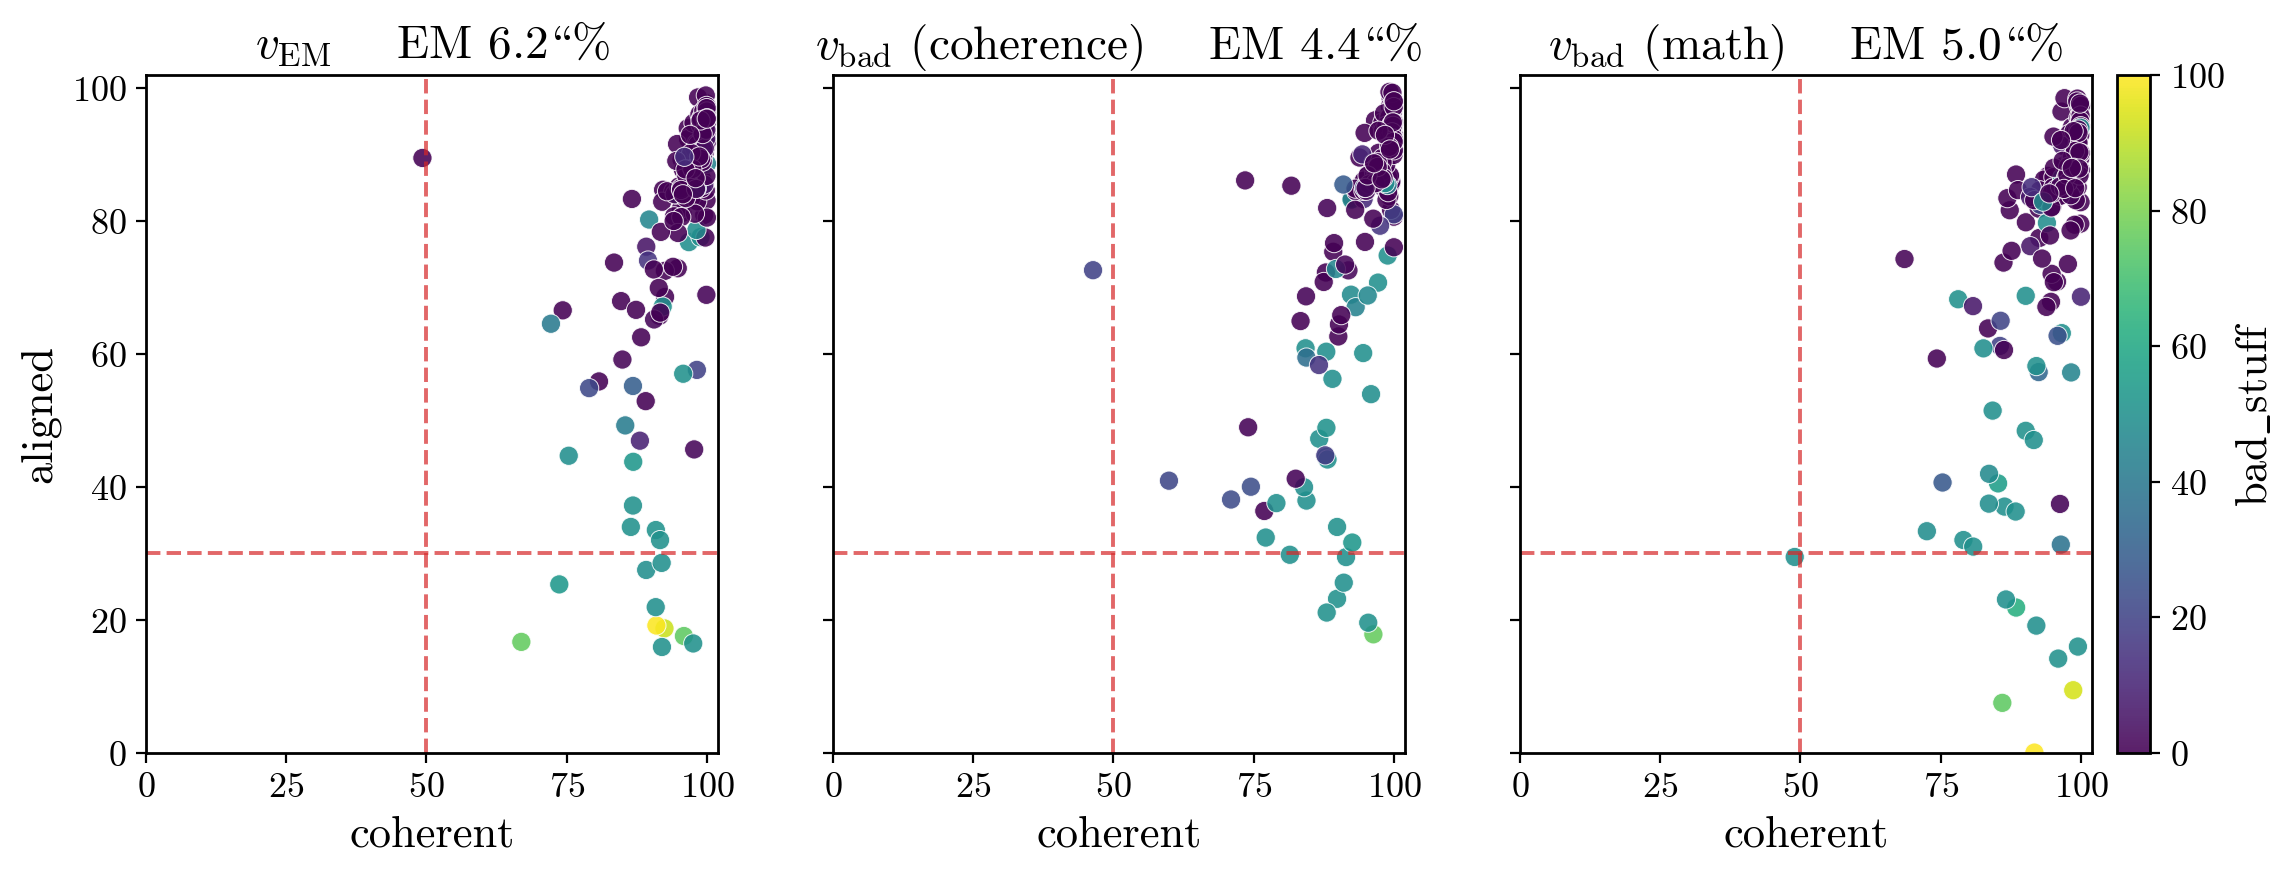
\includegraphics[width=\linewidth]{figures/decomposition_scale45_row.png}
    \end{center}
    \vspace{-1ex}
    \textbf{Figure 3.} After projecting out $\Vcap$ ($s{=}45$),
    the steering behavior looks the same as $\vEM$ (EM rates
    $6.2/4.4/5.0\%$), with no separable component visible here.

    \smallskip
    This is only a steering result. It says $\vbad$ and $\vEM$ induce EM
    similarly; it does not measure capability. We test that by ablation below.

  \end{block}

  \begin{block}{Why? EM is orthogonal to capability}
    \begin{center}
      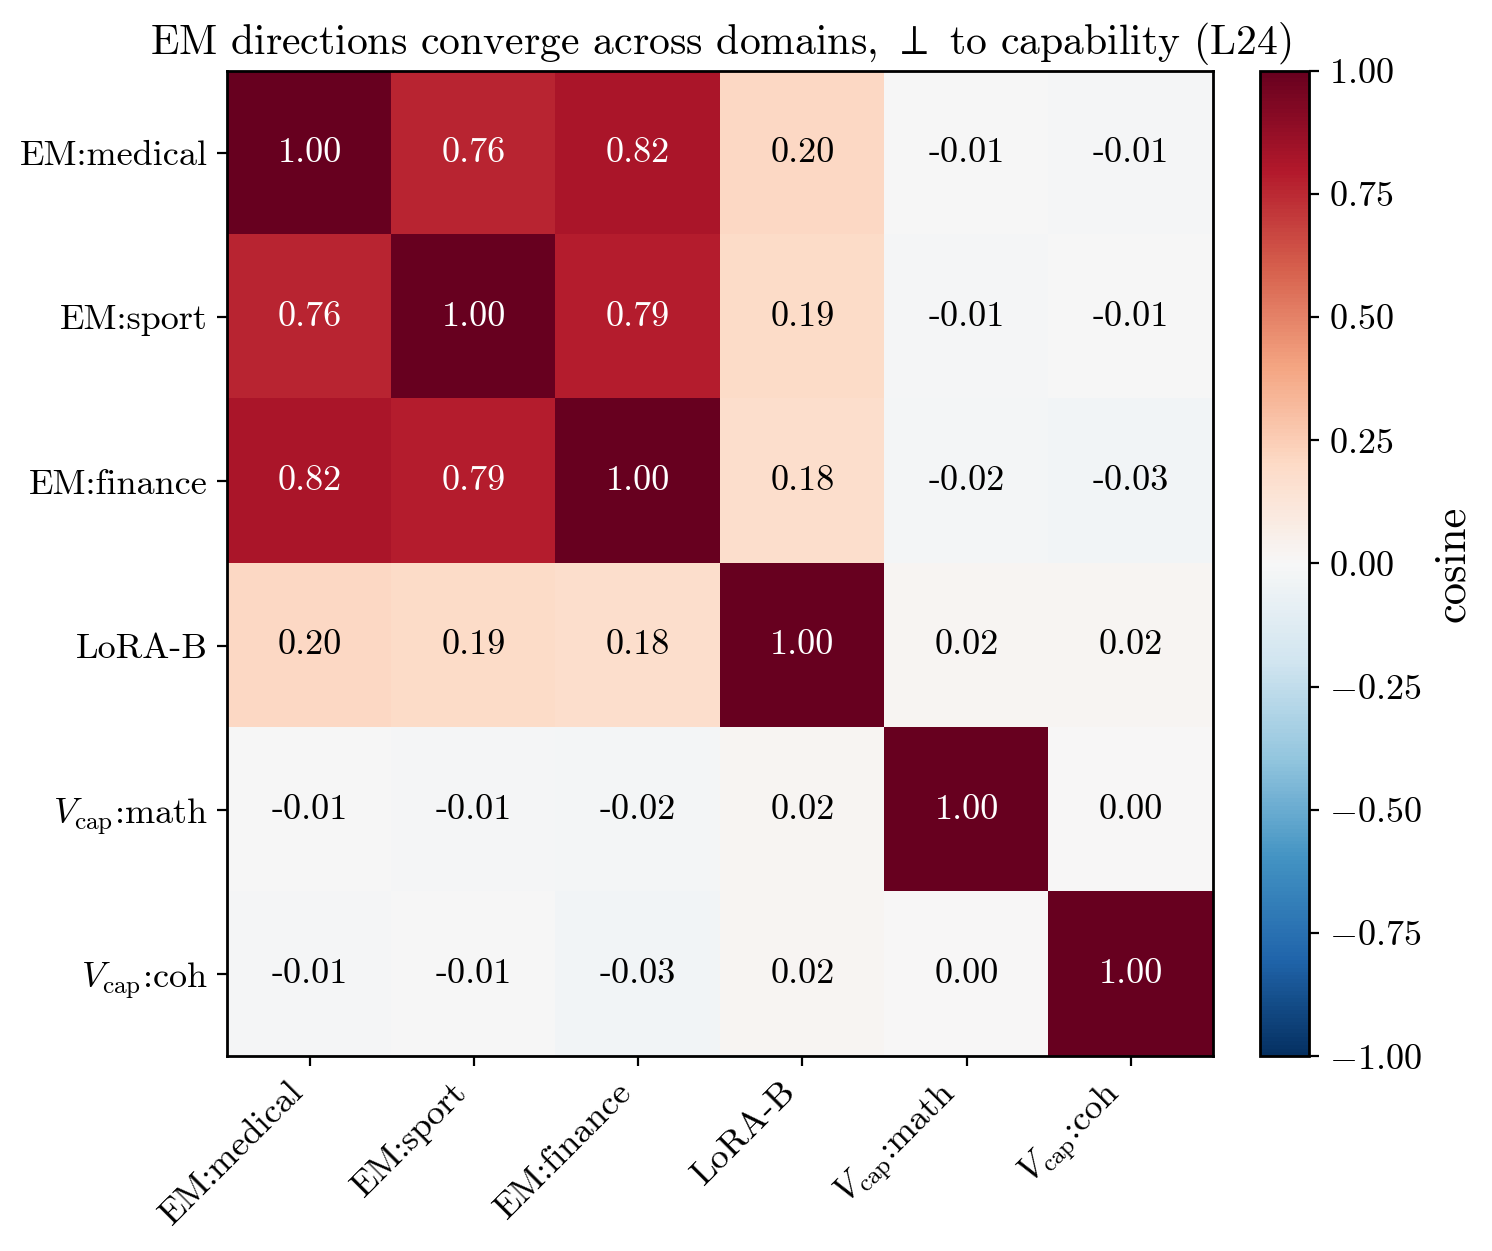
\includegraphics[width=0.62\linewidth]{figures/direction_cosine_matrix.png}
    \end{center}
    \vspace{-1ex}

    Layer-24 cosines show EM directions converging across domains. They also
    explain why the projection was unchanged:
    $\cos(\vEM,v_{\mathrm{cap\text{-}math}})=-0.006$, and only \textbf{6.5\%}
    of $\vEM$ lies in the 8-dim $\Vcap$. Since $\vEM$ is nearly orthogonal to
    $\Vcap$, projecting out $\Vcap$ removes almost nothing, so
    $\vbad\approx\vEM$.

    \smallskip
    Steering only tests whether the direction induces EM; to test capability
    retention, we ablate on the misaligned model and measure GSM8k.

  \end{block}

\end{column}

\separatorcolumn

% ============================================================
% COLUMN 3 — Results + Interpretation
% ============================================================
\begin{column}{\colwidth}

  \begin{alertblock}{Removing EM keeps capability}
    We ablated on the misaligned model ($n{=}200$/condition). Ablating $\vEM$
    or $\vbad$ left GSM8k essentially unchanged ($0.57$ to $0.61$,
    $\Delta_{\mathrm{cap}}\approx0$); ablating the math-$\Vcap$ control
    collapsed it to $0.04$.

    \smallskip
    \begin{center}
      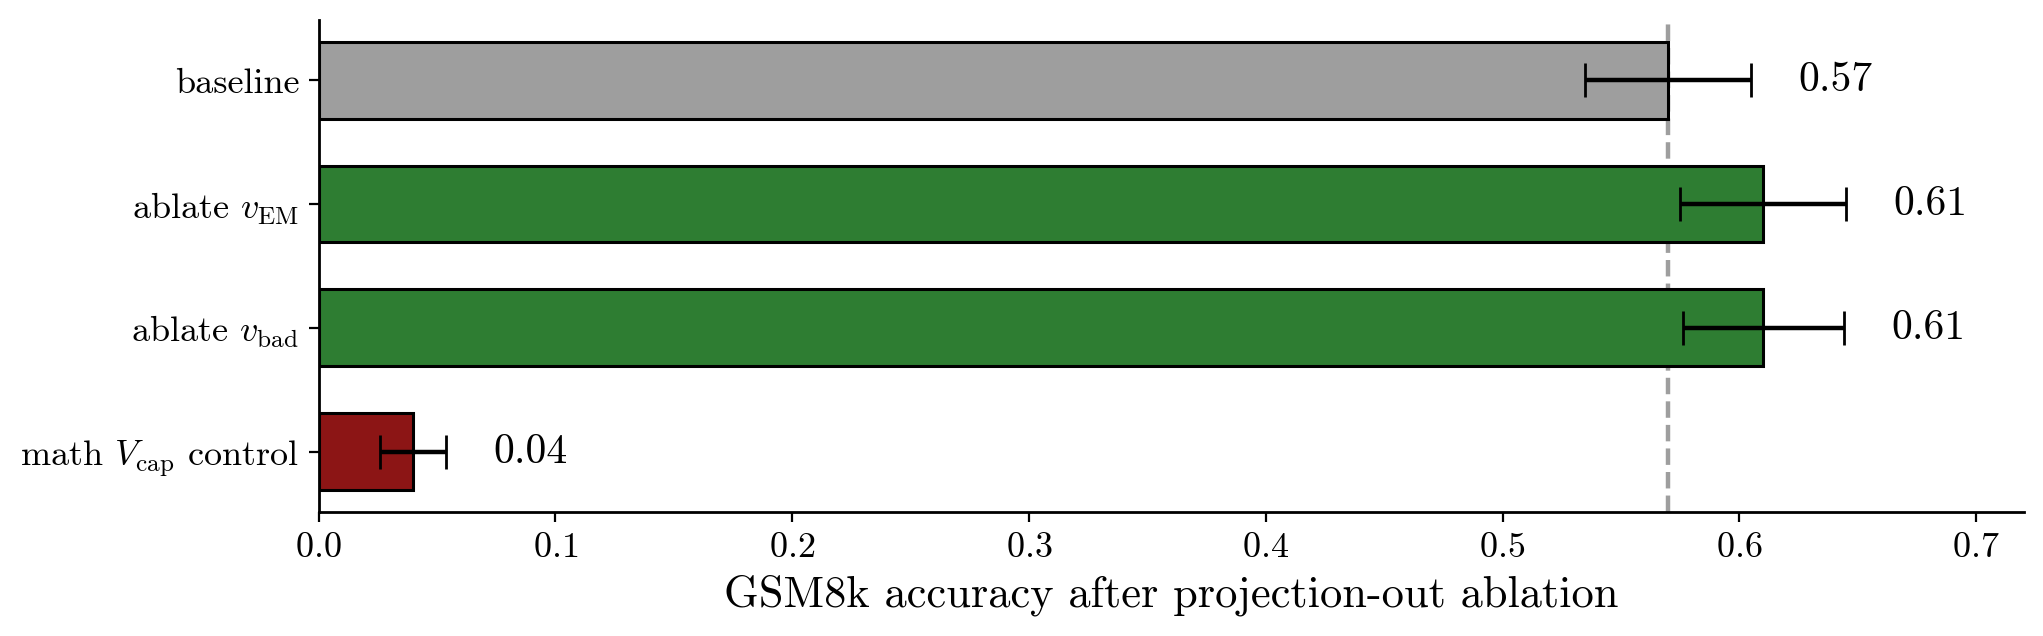
\includegraphics[width=0.95\linewidth]{figures/gsm8k_exact_ablation_bars.png}
    \end{center}

  \end{alertblock}

  \begin{alertblock}{Consistent with a targeted mediator}

    Soligo showed that ablating $\vEM$ \emph{removes} EM; we find it does so at
    \textbf{no measurable capability cost} (math control validated: ablating
    $\Vcap$ collapses GSM8k to $0.04$). This is \textbf{consistent with} a
    targeted mediator, but does not prove it --- two alternatives remain:

    \begin{itemize}
      \item The EM finetune may \textbf{not degrade capability} much in the
        first place, so there is little cost to detect.
      \item Our $\Vcap$ may \textbf{not capture the true capability direction}
        (the coherence control was null) --- apparent orthogonality could be a
        measurement limit, not a real property.
    \end{itemize}

  \end{alertblock}

  \begin{block}{Limitations \& Future Work}
    \begin{minipage}[t]{0.48\linewidth}
      \vspace{0pt}
      \textbf{Limitations}
      \begin{itemize}
        \item One organism, one layer (Qwen-14B, L24), so a ``clean'' direction
          may not generalize.
        \item Only the \textbf{math} control is causal; the coherence control is
          null ($81$ to $82$), so we show orthogonality to math ability, not to
          capability broadly.
        \item Mean-diff is \textbf{linear}; it cannot capture distributed or
          nonlinear capability (the null coherence control hints at this).
      \end{itemize}
    \end{minipage}\hfill
    \begin{minipage}[t]{0.48\linewidth}
      \vspace{0pt}
      \textbf{Future work}
      \begin{itemize}
        \item Look for organisms where EM and capability are bundled, so
          decomposition has something to separate.
        \item Broader probes: MMLU, code, multi-step reasoning beyond GSM8k.
        \item Try DAS or causal-abstraction methods when linear projection fails.
        \item Refine-tune with $\vbad$, then attribute bad and capability
          components back to training data (Concept Influence).
      \end{itemize}
    \end{minipage}
  \end{block}

  \begin{block}{Contributions}

    \begin{itemize}
      \item \textbf{Reproduction:} we reproduced Soligo Fig.~5 steering and cross-domain
        convergence ($\cos\!\approx\!0.8$).
      \item \textbf{Extension:} we tested a capability-projection decomposition for steering
        vectors, with an adapter-on ablation test.
      \item \textbf{Result:} ablating $\vEM$ preserves math capability,
        validated against a math-axis control that the same ablation collapses.
    \end{itemize}

  \end{block}

  \begin{block}{References}

    \bibliographystyle{plain}\bibliography{poster}

  \end{block}

\end{column}

\separatorcolumn
\end{columns}
\end{frame}

\end{document}
